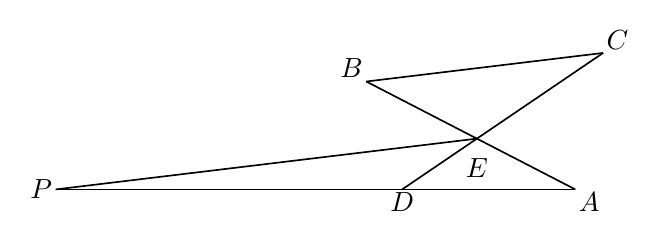
\begin{tikzpicture}[x=1cm,y=1cm,line width=.6pt,font=\normalsize]
\coordinate (P) at (0,0);
\coordinate (D) at (4.4,0);
\coordinate (A) at (6.6,0);
\coordinate (B) at (3.9446,1.3706);
\coordinate (C) at (6.95288,1.73338);
\coordinate (E) at (5.35012,0.6451);
\draw (P)--(A);
\draw (P)--(E);
\draw (B)--(A);
\draw (C)--(D);
\draw (B)--(C);
\node[left,inner sep=1pt] at (P) {$P$};
\node[below,inner sep=1pt] at (D) {$D$};
\node[below right,inner sep=1pt] at (A) {$A$};
\node[above left,inner sep=1pt] at (B) {$B$};
\node[above right,inner sep=1pt] at (C) {$C$};
\node[below=6pt,inner sep=1pt] at (E) {$E$};
\end{tikzpicture}
